\section{Materials and Methods}

\subsection{Polytope representation of the feasible activation space}



\subsection{Hit-and-Run}
The boundaries of the convex polytope defining the feasible activation set are defined by the mechanics of the limb and the constraints of the task, as is described in Subsection \ref{ss:finger}. The goal of the Hit-and-Run algorithm is to uniformly sample  a convex body \cite{smith1984efficient}. 
In the case of a schematic tendon-driven limb with three muscles, the feasible activations start out being the positive unit cube (as muscles can only be activated positively from 0 to a maximal normalized value of 1). As explained in \cite{Valero-Cuevas2009mathematical}, that the feasible activation set for a given static force vector produced at the endpoint of the limb is further reduced by the addition of task constraints  in the form of equality or inequality constraints that define the direction and desired magnitude of the force. Thus if this simple limb is meeting one equality constraint, the feasible activation set os the polygon $P$ containing all feasible activation  $\textbf{a} \in \mathbb{R}^n$ that satisfy
\[\textbf{f} = A\textbf{a}, \textbf{a} \in [0,1]^n,\]
where $\textbf{f} \in \mathbb{R}^m$ is a fixed force vector and $A = J^{-T}RF_m \in \mathbb{R}^{m \times n}$---the matrices of the Jacobian of the limb, the moment arms of the tendons, and the strengths of the muscles, respectively \cite{Valero-Cuevas1998Large,Valero-Cuevas2009mathematical}. $P$ is bounded by the unit $n$-cube since all variables $a_i$, $i \in [n]$ are bounded by 0 and 1 from below, above respectively.
Consider the following $1 \times 3$ fabricated example.
\begin{align*}
&1 = \frac{10}{3}a_1 - \frac{53}{15}a_2 + 2a_3 \\
&a_1, a_2, a_3 \in [0,1],
\end{align*}
the set of feasible activations is given by the shaded set in Figure \ref{fig_hr}.

\begin{figure}[ht]
  %\sidecaption
\end{figure}
   \begin{center}
    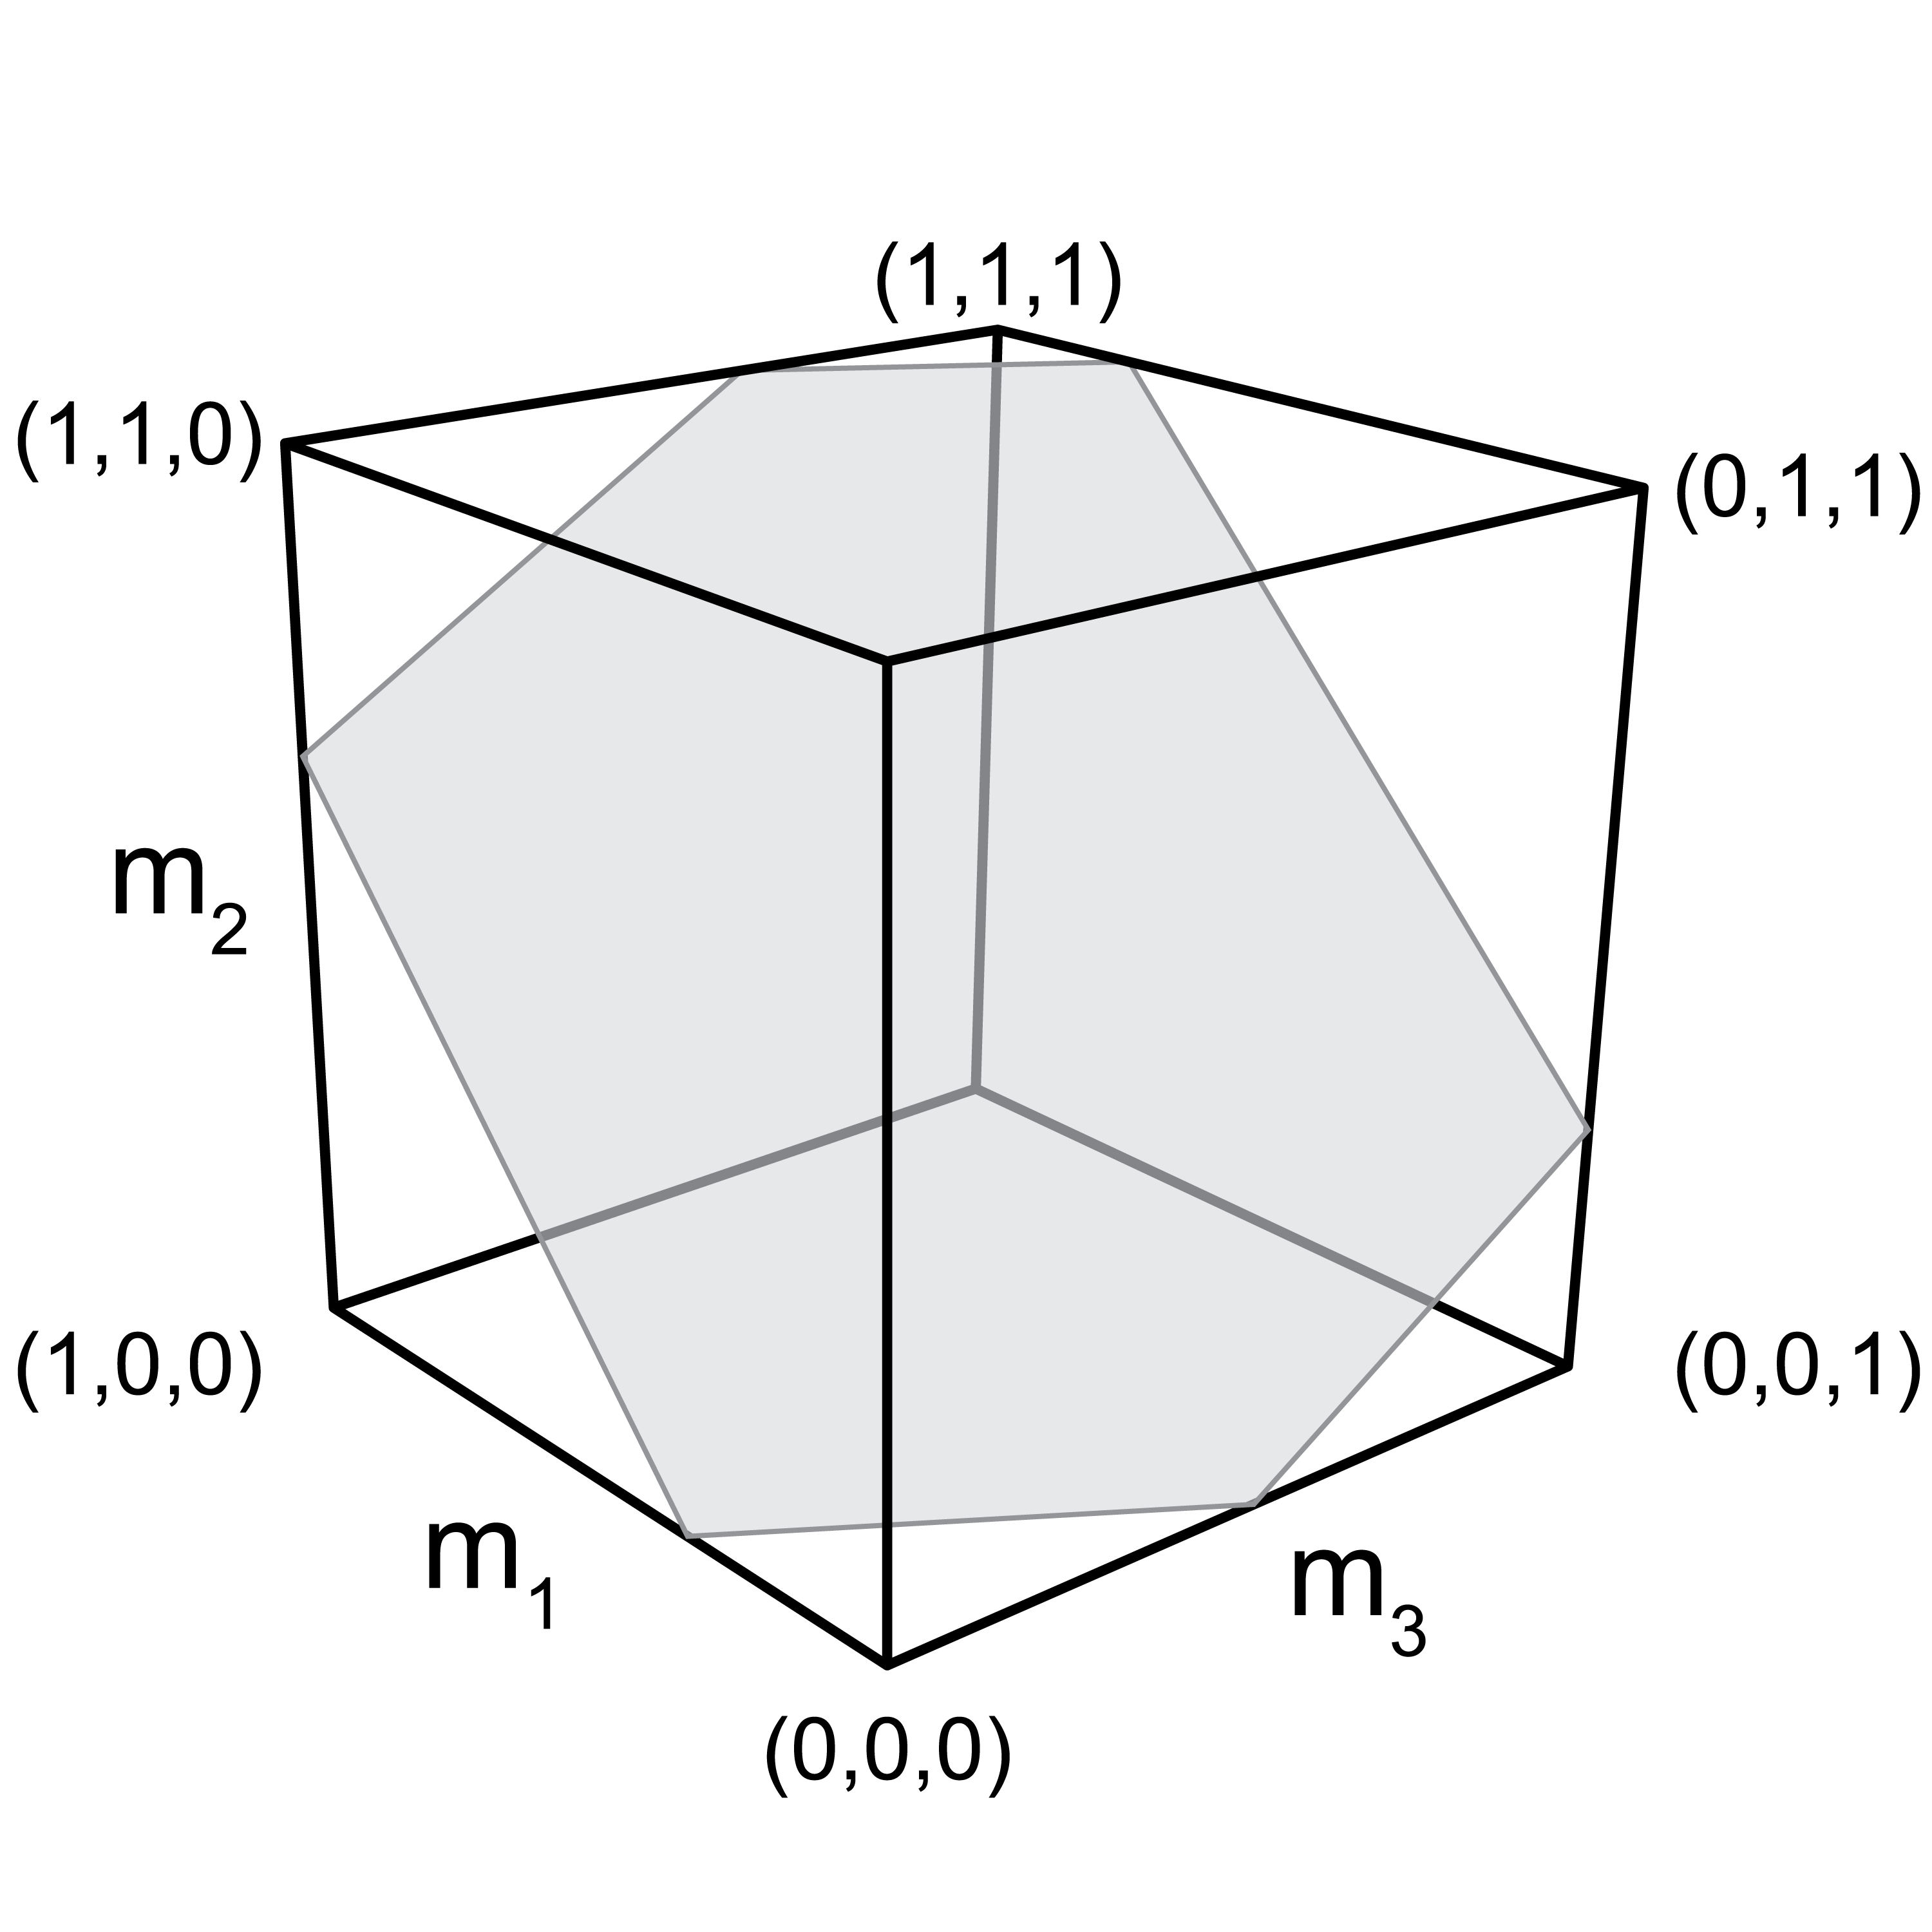
\includegraphics[width=0.25\textwidth]{sections/figs/feasibleactivation.png}
  \end{center}
  \caption{The feasible activation set for a  three-muscle system meeting one functional constraint is a polygon in $\mathbb{R}^3$. Note that muscle activations are assumed to be bounded between $0$ and $1$.}
  \label{fig_hr}
\end{figure}

The Hit-and-Run walk on $P$ is defined as follows (it works analogously for any convex body). 
\begin{enumerate}
\item Inner Point: Find a given starting point $\textbf{p}$ of $P$ (Figure \ref{fig:hitruncube}(a)) .
\item Direction: Generate a random direction through $\textbf{p}$ (uniformly at random over all directions) (Figure \ref{fig:hitruncube}(b)).
\item Endpoints: Find the intersection points of the random direction with the $n$-unit cube (Figure \ref{fig:hitruncube}(c)).
\item New Point: Choose the next point of the sampling algorithm uniformly at random from the segment of the line in $P$ (Figure \ref{fig:hitruncube}(d)). 
\item Repeat from $(b)$ the above steps with the new point as the starting point .
\end{enumerate}

How many steps are necessary to reach a uniformly at random point in the polytope? For convex polygons in higher dimensions, experimental results suggest that $\mathcal{O}(n)$ steps of the Hit-and-Run algorithm are sufficient. In particular Emiris and Fisikopoulos paper suggest that $(10 + 10\frac{n})n$ steps are enough to have a close to uniform distribution \cite{emiris2013efficient}.
Therfore for given output force we execute the Hit-and-Run algorithm 1000 times on 100 points. The experimental results propose that those 1000 points are uniformly distributed on the polygon.

\subsection{Starting Point}
To find a starting point in 
\[\textbf{f} = A\textbf{a}, \textbf{a} \in [0,1]^n,\]
we only need to find a feasible activation vector. For the hit and run algorithm to mix faster, we do not want the starting point to be in a vertex of the activation space. We use the following standard trick using slack variables $\epsilon_i$.

\begin{equation}\label{eq:LP_r}
\begin{array}{lrcl}
\mbox{maximize} & \sum_{i=1}^n \epsilon_i \\ 
\mbox{subject to} & \textbf{f} &=& A\textbf{a}\\
  & a_i &\in& [\epsilon_i, 1- \epsilon_i], \hspace{5mm} \forall i \in \{1,\dots,n\}  \\
  & \epsilon_i &\geq& 0, \hspace{5mm} \forall i \in \{1,\dots,n\}.  
\end{array}
\end{equation}

\subsection{Realistic index finger model}
\label{ss:finger}
We began with an index finger of a healthy human (male) right hand, which was taken from [JOB 1998]. The hand size, finger lengths, and weight was []. Experimental forces from []. 
The moment arm matrix, $R$, which contains the leverage of each tendon's insertion points across each joint, was measured by doing [], [] ,and then [].
The Jacobian, $J$, which represents the effect of rotation at each DOF on each component of endpoint wrench [cite jacobian usage], was measured with a [], by [], with precision of $\pm x$.
The force-naught vector, $F_0$, which contains the tendon force at maximal isometric contration (MIC)[cite method used] for each muscle, was taken in the [same or different] posture, with a [] measuring device, with precision of $\pm x$.

